\chapter{Teori} %HUSK KILDER
\section{Længde- og breddegrader}
I et geografisk koordinatsystem, er jorden inddelt i længde- og breddekredse. Idet jorden er rund, er disse længde- og breddekredse målt i grader, og de bliver i stedet kaldt længde- og breddegrader. 
Længdegrader beskriver de vertikale linjer på verdenskortet i figur 5.1, som går fra nordpolen til sydpolen. Disse bliver også betegnet som meridianer. Meridianen der går gennem Greenwich kaldes nulmeridianen, hvorefter den første vestlige længdegrad bliver udtrykt som 1 grad vestlig længde, og det samme gælder for den første østlige længdegrad, som vil være 1 grad østlig længde. Disse længdegrader bliver herefter talt op, i hver deres retning. Idet en cirkel er 360 grader, er de sidste meridianer på hver sin side af verdenskortet kaldet 180 grader østlig/vestlig længde, da 180 er det halve af 360. Det skal desuden også nævnes, at længdekredsene ikke nødvendigvis har den samme afstand, da længdekredsene har mindre indbyrdes afstand jo tættere på polerne de er. 
Breddegrader beskriver de horisontale linjer i verdenskortet nedenunder. Disse linjer er parallelle med ækvator, og deres indbyrdees afstand bliver derfor hverken mindre eller større, men deres omkreds bliver kortere alt efter hvor tæt på polerne de befinder sig.
\begin{figure} [h]
	\centering
	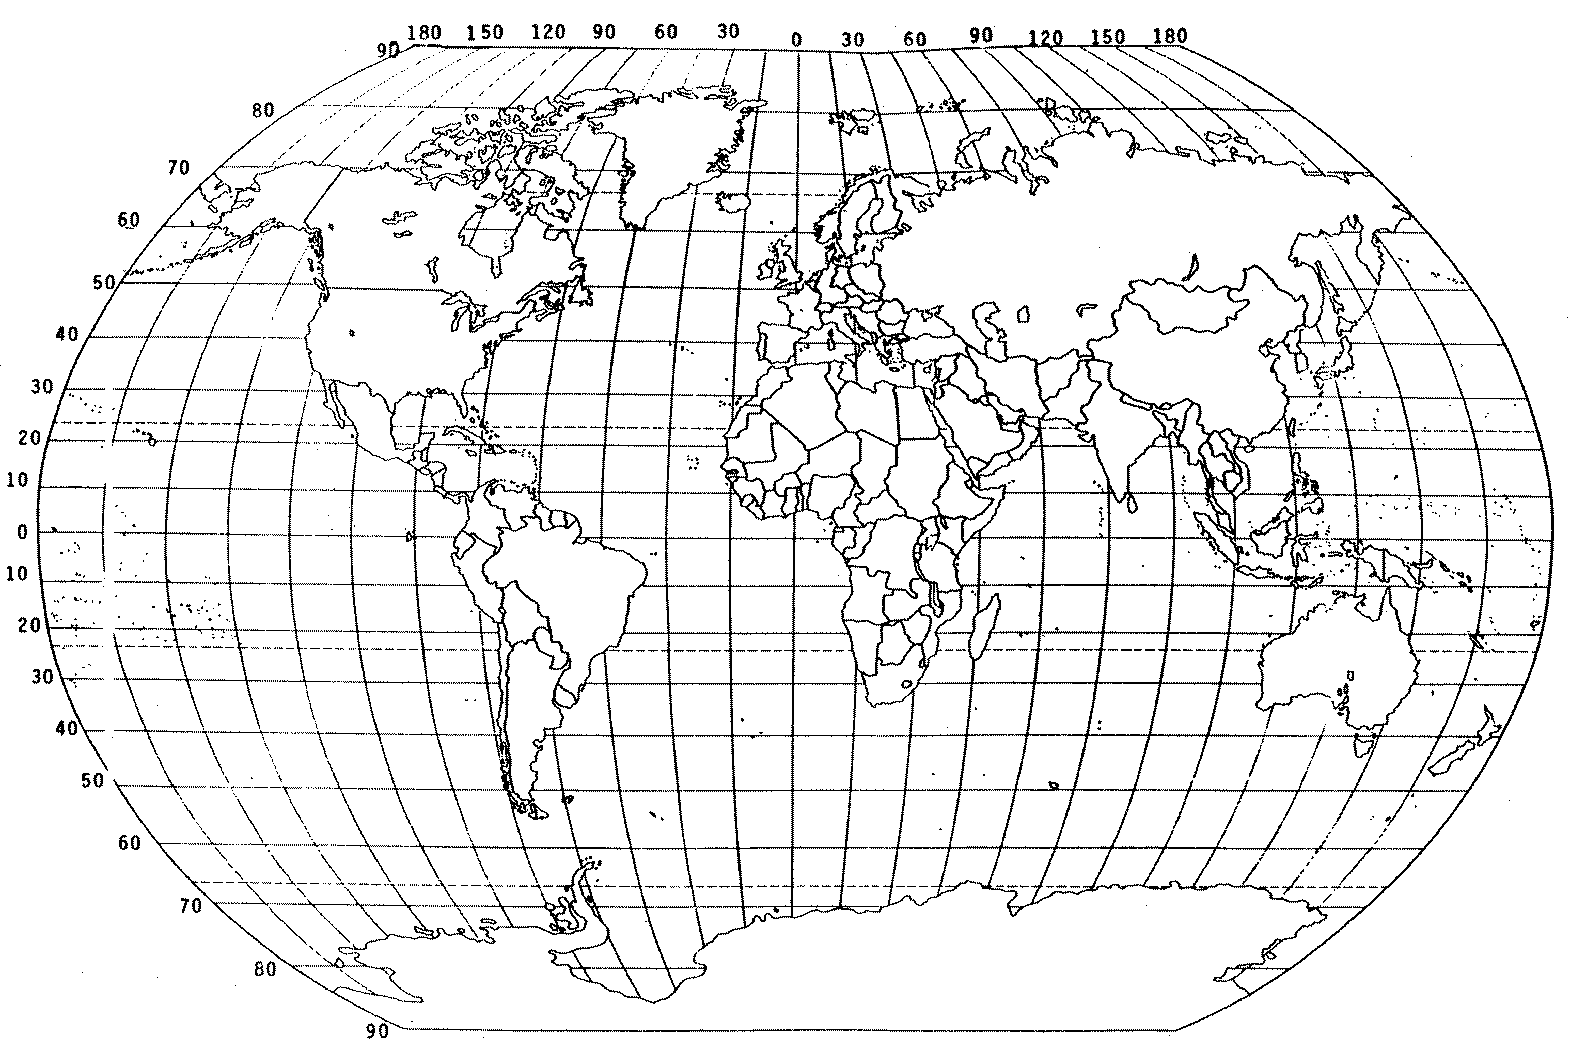
\includegraphics[width=.5\textwidth]{billeder/longlatmap}
	\caption{Verdenskort med længde- og breddegrader}
\end{figure}

Når der ønskes fundet en lokalitet vha. længde- og breddegrader, er det meget simpelt, den længdegrad der bliver oplyst, skal man først finde på verdenskortet, hvorefter den oplyste breddegrad skal findes. Når begge er fundet, er den ønskede lokalitet fundet. Et simpelt eksempel kunne være, at byen Aalborg ønskes fundet, vha. længde- og breddegrader. Ved at benytte Danmarkskortet nedenunder på figur 5.2, kan det aflæses, at Aalborg tilnærmelsesvis har koordinaterne 57o N og 10o E. Hvis disse koordinater ønskes meget præcist, er der diverse muligheder online, som Google Maps og lignende der kan aflæse dette meget præcist, ellers skal der anskaffes et kort i mindre målestoksforhold, over f.eks. Nordjylland eller endnu mindre.  
\begin{figure} [h]
	\centering
	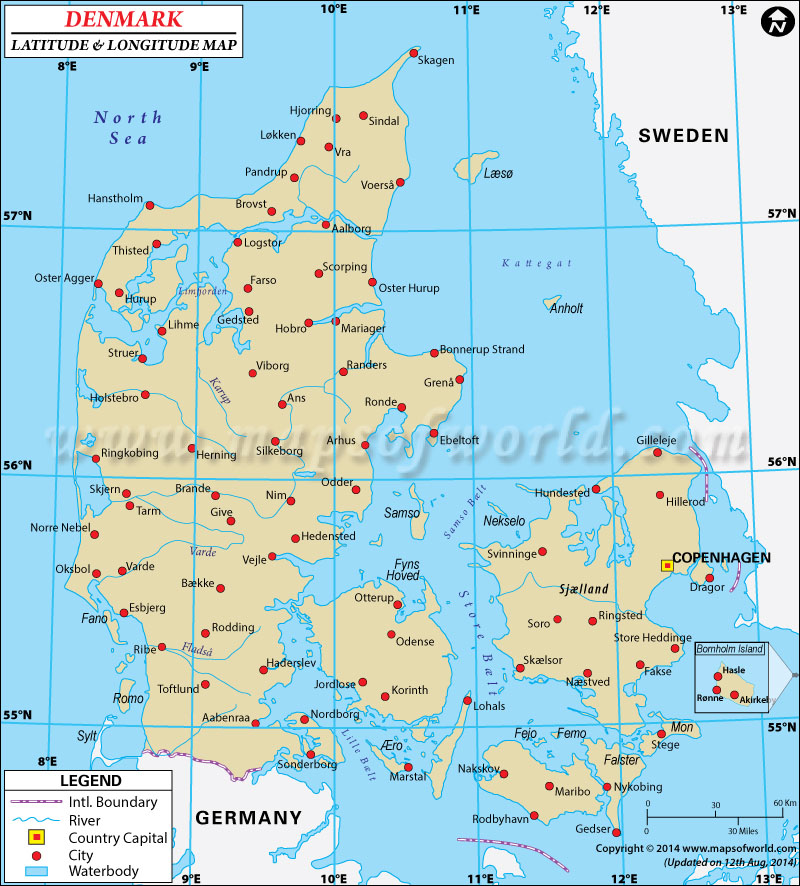
\includegraphics[width=.4\textwidth]{billeder/long-lat-denmark}
	\caption{Danmarkskort med længde- og breddegrader}
\end{figure}

\section{Universal Transverse Mercator Projektion}
Universal Transverse Mercator Projektion, forkortet UTMP, er en måde at opdele jordkloden på, og derved udforme koordinatsæt for, hvor noget befinder sig henne. Denne metode gør brug af, at jordkloden, som reelt set er rund, bliver omformet til en flade, ligesom et stykke papir. Her bliver jorden inddelt i 60 zoner, hvor hver zone er opdelt, startende fra 180 meridianen, og regnes fra vest til øst. Jorden er indelt mellem 80° S bredde, og 84° N bredde, der breskriver 60 zoner, hvor hver zones vidde er 6°. Zonerne er nummereret efter deres placering ift. start-zonen (mest vestlige).
Alle zonerne i UTM systemet er baseret på en Transverse Mercator projektion, som ikke vil blive yderligere beskrevet i denne rapport, hvor en region kan kortlægges uden stor forvrængning af jordklodens ellers runde form. Hvis jorden blev kortlagt i én stor region, vil dette forårsage store afstandsfejlberegninger, da der ikke vil blive taget højde for jordklodens runde form. Det er her at Transverse Mercator projektionen er smart, da den sørger for en lav grad af forvrængning, da det er smalle breddegrader (6°) der typisk anvendes til zonerne. 
Ved positionering gennem UTM systemet, oplyses følgende: Først en længdezone fra UTM, dernæst afstanden fra zonens central median, herefter en nordlig afstand, som zonens projekterede afstand fra ækvator.


\subsection{Opsummering}

